\documentclass[conference]{IEEEtran}
\IEEEoverridecommandlockouts
% The preceding line is only needed to identify funding in the first footnote. If that is unneeded, please comment it out.
\usepackage{cite}
\usepackage{amsmath,amssymb,amsfonts}
\usepackage{algorithmic}
\usepackage{graphicx}
\usepackage{textcomp}
\usepackage{xcolor}
\def\BibTeX{{\rm B\kern-.05em{\sc i\kern-.025em b}\kern-.08em
		T\kern-.1667em\lower.7ex\hbox{E}\kern-.125emX}}
\usepackage{url}
\usepackage{booktabs}

\usepackage{tikz}
\usetikzlibrary{shapes.geometric, arrows}
\tikzstyle{startstop} = [circle, radius=3cm, text centered, draw=black, fill=red!30]
\tikzstyle{io} = [trapezium, trapezium left angle=70, trapezium right angle=110, minimum width=3cm, minimum height=1cm, text centered, text width=3cm, draw=black, fill=blue!30]
\tikzstyle{process} = [rectangle, minimum width=3cm, minimum height=1cm, text width=3cm, text centered, draw=black, fill=orange!30]
\tikzstyle{decision} = [diamond, minimum width=3cm, minimum height=1cm, text centered, draw=black, fill=green!30]
\tikzstyle{arrow} = [thick,->,>=stealth]

\begin{document}
	
\title{Optimization Using Method of Exhaustive Search, Greedy Search and MATLAB's solver}
	
\author{
	\IEEEauthorblockN{John Michael P. Corbeta\textsuperscript{*}, Abdul Aziz G. Mabaning\textsuperscript{$\dagger$}}
	\IEEEauthorblockA{\textit{Department of Electrical Engineering, College of Engineering and Technology} \\
		\textit{Mindanao State University - Iligan Institute of Technology}\\
		Iligan City, Philippines \\
		\textsuperscript{*}johncorbeta1997@gmail.com, \textsuperscript{$\dagger$}mraaguevarra@gmail.com}
}
	
\maketitle

\begin{abstract}
	There are many fields in power systems that requires optimizations. Power system optimization ranges from continuous problems like economice dispatch to complex decision making of unit commitment. This paper discusses the pros and cons of the following optimization methods: exhaustive search, greedy search, and MATLAB/Octave solver. These methods will be implemented into a optimal placement problem for phasor measurement units (PMUs) in IEEE test sytems for power system estimation.
\end{abstract}

\begin{IEEEkeywords}
	Power system optimization, matlab, octave, exhaustive search, greedy algorithm
\end{IEEEkeywords}

\section{Introduction}
Monitoring the state of the power system is one of the important applications of power system optimization. This provides accurate understanding and data of the current state of power system operation. This requires measurement datas from measuring and communication devices located all throughout the power system. This devices, remote terminal units (RTUs) and PMUs provide measurement datas of their respective buses to the control center. PMUs are devices which uses synchronization signals from global positional system (GPS) satellites and provide positive sequence phasor voltages and currents measured at a given substation improving the performance of state estimators. This study refers to the pioneering work in optimal PMU placement (OPP) by Phadke et al. \cite{Phadke1986,Phadke1993} and its relaxed constraints to a simplified state estimator in \cite{Baldwin1993}. This problem is formulated and solved using Octave's linear programming solver, exhaustive/brute search, and greedy algorithm.

GNU Octave is a software featuring high-level programming language primarily intended for numerical computation. Octave helps in solving linear and nonlinear problems numerically, and for performing other numerical experiments using a language that is mostly compatible with MATLAB. On the other hand, brute-force search or exhaustive search, also known as generate and test, is a very general problem-solving technique and algorithmic paradigm that consists of systematically enumerating all possible candidates for the solution and checking whether each candidate satisfies the problem's statement. While a brute-force search is simple to implement and will always find a solution if it exists, implementation costs are proportional to the number of candidate solutions, which in many practical problems tends to grow very quickly as the size of the problem increases\cite{EmilyFox}. Therefore, brute-force search is typically used when the problem size is limited, or when there are problem-specific heuristics that can be used to reduce the set of candidate solutions to a manageable size. The method is also used when the simplicity of implementation is more important than speed. Greedy algorithm however, is any algorithm that follows the problem-solving heuristic of making the locally optimal choice at each stage. Greedy heuristics are known to produce suboptimal results on many problems, \cite{Feige1998} and so natural questions are:
\begin{itemize}
	\item For which problems do greedy algorithms perform optimally?
	\item For which problems do greedy algorithms guarantee an approximately optimal solution?
	\item For which problems are the greedy algorithm guaranteed not to produce an optimal solution?
\end{itemize}
A large body of literature exists answering these questions for general classes of problems, such as matroids\cite{Nishimura2009}, as well as for specific problems\cite{Chvatal1979}, such as set cover.

This paper discusses the effectiveness of these methods in solving an optimial PMU place ment problem. An IEEE 7-bus system will be used in analyzing the constraints of the optimization problem. The methods will then be implemented into larger IEEE test systems.

\section{Problem Formulation}
A PMU placed at a given bus is capable of measuring the voltage phasor of the bus as well as the phasor currents for all lines incident to that bus. Thus, the entire system can be made observable by placing PMUs at strategic buses in the system. The objective of the OPP problem is to
accomplish this task by using a minimum number of PMUs.

For an n-bus system, assuming an equal cost of all PMU installation, the cost of PMU placement would be irrelevant for the optimization problem. Thus only the number of PMUs is considered, the PMU placement problem can be formulated as follows:
\begin{gather}
	\text{min}\hspace{2mm}c(\mathbf{x})=\sum_{i=1}^{n}x_i \\
	\text{s.t.}\hspace{2mm}\mathbf{f}(\mathbf{x}) \geq \hat{1}
\end{gather}
where $\mathbf{x}$ is a binary decision variable vector, whose entries are defined as:
\begin{equation}
	x_i=\begin{cases}
		1 & \text{is a PMU is installed in bus $i$} \\
		0 & \text{otherwise}
		\label{eq:x}
	\end{cases}
\end{equation}
$\mathbf{f}(\mathbf{x})$ is a vector function whose entries are non-zero if the corresponding bus voltage is solvable using the given measurement set and zero otherwise while $\hat{1}$ is a vector whose entries are all ones. Consider the 7-bus system and its measurement configuration shown in Figure.
\begin{figure}[htbp]
	\includegraphics[width=\columnwidth]{fig2.1.png}
	\caption{IEEE 7-bus system}
	\label{fig:ieee7}
\end{figure}
First, form the binary connectivity matrix $A$. The entries of $A$ are defined as follows:
\begin{equation}
	A_{j,k} = \begin{cases}
		1 &\text{if}\hspace{1mm}Y_{j,k} \neq 0 \\
		0 &\text{if otherwise}
	\end{cases}
\end{equation}

Matrix A can be directly obtained from the bus admittance matrix by transforming its entries into binary form. Building
the A matrix for the 7-bus system of Figure yields:
\begin{equation}
	\mathbf{A} = \begin{bmatrix}
		1 &1 &0 &0 &0 &0 &0 \\
		1 &1 &1 &0 &0 &1 &1 \\
		0 &1 &1 &1 &0 &1 &0 \\
		0 &0 &1 &1 &1 &0 &1 \\
		0 &0 &0 &1 &1 &0 &0 \\
		0 &1 &1 &0 &0 &1 &0 \\
		0 &1 &0 &1 &0 &0 &1 \\
	\end{bmatrix}
\label{eq:A}
\end{equation}
The constraints for this case can be formed as the product of matrix $\mathbf{A}$ and solution vector $\mathbf{x}$ in (\ref{eq:fx}).
\begin{equation}
	\mathbf{f}(\mathbf{x}) = \mathbf{A} \cdot \mathbf{x} \geq \hat{1}
	\label{eq:fx}
\end{equation}

\subsection{Exhaustive/Brute Search}
In this subsection, the framework for exhaustive/brute search is designed. Exhaustive search has the computation time in solving optimization problem. It collects all possible solution in finding the optimal objective value. For an OPP problem of an $n$ bus system, with each $x_i$ having the two possible value as described in (\ref{eq:x}), the number of possible solution is as follows:
\begin{equation}
	m = 2^n-1
\end{equation}
Each solution $k$ is then evaluated to the current optimal solution $\hat{\mathbf{x}}$ where:
\begin{align}
	c(\mathbf{x}^{(k)})<c(\hat{\mathbf{x}}) &\rightarrow \text{$\mathbf{x}^{(k)}$ is optimal} \label{eq:brute1} \\
	c(\mathbf{x}^{(k)})=c(\hat{\mathbf{x}})&\rightarrow \text{$\mathbf{x}^{(k)}$ is cooptimal} \label{eq:brute2} \\
	c(\mathbf{x}^{(k)})>c(\hat{\mathbf{x}}) &\rightarrow \text{$\mathbf{x}^{(k)}$ is not optimal} \label{eq:brute3}
\end{align}
In (\ref{eq:brute1}-\ref{eq:brute3}), brute search algorithm for OPP problem can obtain more than one solution, cooptimal solutions. The algorithm can be modified to record all the possible solution and respected value by eliminating the condition of optimality and sorting the record of solutions. Looking for the next optimal solution from the previously found solution adds complexity to the algorithm. In order to do so , we must add the solution to the constraints as shown in (\ref{eq:Anew}) and (\ref{eq:fnew}). The algorithm for the brute search algorithm is depicted in Fig. \ref{fig:brute}.
\begin{gather}
	\mathbf{A}_{new} = \begin{bmatrix}
		\mathbf{A}_{old} \\
		1-\hat{\mathbf{x}}
	\end{bmatrix} \label{eq:Anew}\\
	\mathbf{f}(\mathbf{x})_{new} = \mathbf{A}_{new} \cdot \mathbf{x} \geq \hat{1} \label{eq:fnew}
\end{gather}

The importance in obtaining cooptimal and sub-optimal solution is to have viable options in case we are restricted in using the global optimum for some reasons like geological or economical.

\begin{figure}
	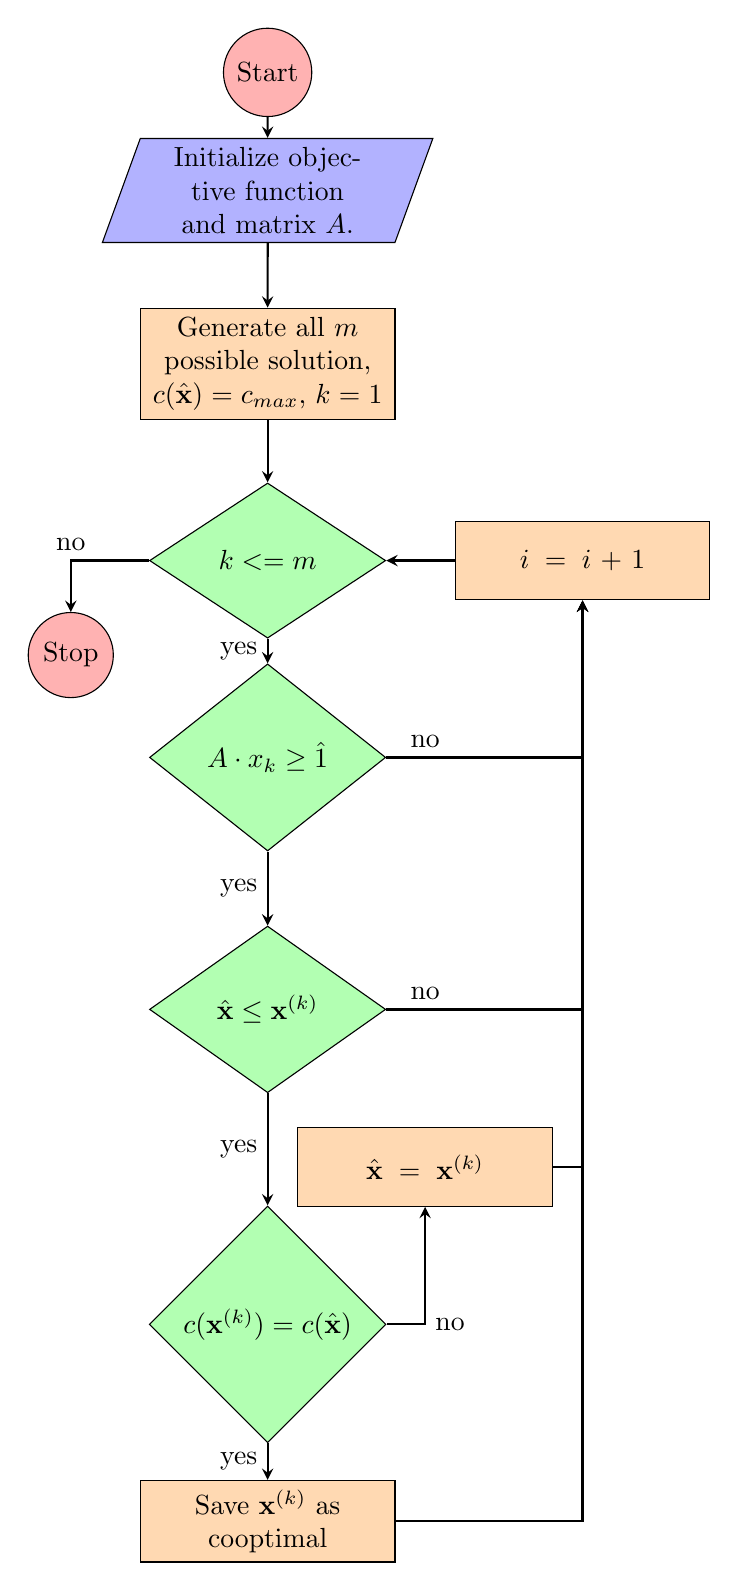
\begin{tikzpicture}[node distance=1.5cm]
		\node (start) [startstop] {Start};
		\node (in1) [io,below of=start] {Initialize objective function and matrix $A$.};
		\node (pro1) [process,below of=in1,yshift=-0.7cm] {Generate all $m$ possible solution, $c(\hat{\mathbf{x}})=c_{max}$, $k=1$};
		\node (dec1) [decision,below of=pro1,yshift=-1cm] {$k<=m$};
		\node (dec2) [decision,below of=dec1, yshift=-1cm] {$A \cdot x_k \geq \hat{1}$};
		\node (dec3) [decision,below of=dec2,yshift=-1.7cm] {$\hat{\mathbf{x}}\leq\mathbf{x}^{(k)}$};
		\node (dec4) [decision,below of=dec3,yshift=-2.5cm] {$c(\mathbf{x}^{(k)})=c(\hat{\mathbf{x}})$};
		\node (pro2) [process,below of=dec4,yshift=-1cm] {Save $\mathbf{x}^{(k)}$ as cooptimal};
		\node (pro3) [process,right of=dec1,xshift=2.5cm] {$i=i+1$};
		\node (stop) [startstop,left of=dec1,xshift=-1cm,yshift=-1.2cm] {Stop};
		\node (pro4) [process,right of=dec4,xshift=0.5cm,yshift=2cm] {$\hat{\mathbf{x}}=\mathbf{x}^{(k)}$};
		\draw [arrow] (start) -- (in1);
		\draw [arrow] (in1) -- (pro1);
		\draw [arrow] (pro1) -- (dec1);
		\draw [arrow] (dec1) -- node[anchor=east] {yes} (dec2);
		\draw [arrow] (dec2) -- node[anchor=east] {yes} (dec3);
		\draw [arrow] (dec3) -- node[anchor=east] {yes} (dec4);
		\draw [arrow] (dec4) -- node[anchor=east] {yes} (pro2);
		\draw [arrow] (pro2) -| (pro3);
		\draw [arrow] (dec3) -| node[anchor=south,xshift=-2cm] {no} (pro3);
		\draw [arrow] (dec2) -| node[anchor=south,xshift=-2cm] {no} (pro3);
		\draw [arrow] (pro3) -- (dec1);
		\draw [arrow] (dec1) -| node[anchor=south] {no} (stop);
		\draw [arrow] (dec4) -| node[anchor=west] {no} (pro4);
		\draw [arrow] (pro4) -| (pro3);
	\end{tikzpicture}
	\caption{Brute force algorithm for optimal PMU placement}
	\label{fig:brute}
\end{figure}

\subsection{Greedy Algorithm}
The greedy algorithm is a multi-stage optimization that involves decision making of selecting the optimum value of each variable to obtain the overall optimum of the system. Considering Fig. \ref{fig:ieee7}, in order to obtain the minimum number of PMUs to be installed, each PMU must observe as much buses as it can. Thus the single stage process of the greedy method is to select the PMU that can observe the maximum buses. Now the buses to be observed are the constraints of the OPP, therefore each stage maximizes the constraints covered by $\hat{x_i}=1$. We must first initialize our solution as $\hat{\mathbf{x}}=\hat{0}$. Looking closely at (\ref{eq:A}), the columns represent each sample variable $\hat{x}_i$. For the first stage, the sum of the elements of the column is the number of constraints covered by each variable given by (\ref{eq:stage1}).
\begin{equation}
	\label{eq:stage1}
	\text{sum}(\mathbf{A},\downarrow) = \begin{bmatrix}
		2 &5 &4 &4 &2 &3 &3
	\end{bmatrix}
\end{equation}

From (\ref{eq:stage1}), 5 at column 2 is the maximum value, thus $\hat{x_2}=1$. For stage 2, we repeat stage 1 but exclude $\hat{x_2}$ from the process. This time we need to create a filter vector to multiply to the rows $\mathbf{A}$ matrix. This filter vector $\mathbf{g}$ can be derived as follows:
\begin{equation}
	\mathbf{g} = 1-\hat{\mathbf{x}}
	\label{eq:filter}
\end{equation}
Filter vector from (\ref{eq:filter}) guarantees that the sum for column 2 is zero. The sum for stage 2 is as follows:
\begin{equation}
	\text{sum}(\mathbf{A},\downarrow) = \begin{bmatrix}
		0 &0 &1 &2 &2 &0 &1
	\end{bmatrix}
\end{equation}
In this case either $\hat{x}_4$ of $\hat{x}_5$ is selected. This process is repeated until the all $m$ constraints are covered. Searching for other solutions is also possible with (\ref{eq:Anew}). This algorithm is depicted in Fig. \ref{fig:greedy}.
\begin{figure}
	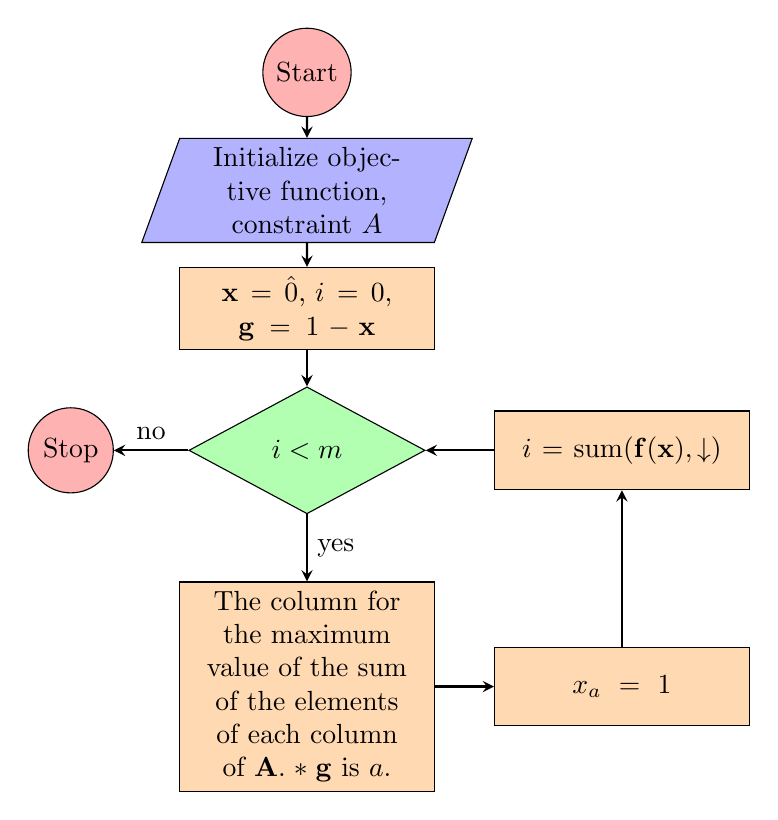
\begin{tikzpicture}[node distance=1.5cm]
		\node (start) [startstop] {Start};
		\node (in1) [io,below of=start] {Initialize objective function, constraint $A$};
		\node (pro1) [process,below of=in1] { $\mathbf{x}=\hat{0}$, $i=0$, $\mathbf{g}=1-\mathbf{x}$};
		\node (dec1) [decision,below of=pro1,yshift=-0.3cm] {$i < m$};
		\node (pro2) [process,below of=dec1,yshift=-1.5cm] {The column for the maximum value of the sum of the elements of each column of $\mathbf{A}.*\mathbf{g}$ is $a$.};
		\node (pro3) [process,right of=pro2,xshift=2.5cm] {$x_a=1$};
		\node (pro4) [process,right of=dec1,xshift=2.5cm] {$i = \text{sum}(\mathbf{f}(\mathbf{x}),\downarrow)$};
		\node (stop) [startstop,left of=dec1,xshift=-1.5cm] {Stop};
		\draw [arrow] (start) -- (in1);
		\draw [arrow] (in1) -- (pro1);
		\draw [arrow] (pro1) -- (dec1);
		\draw [arrow] (dec1) -- node[anchor=west] {yes} (pro2);
		\draw [arrow] (pro2) -- (pro3);
		\draw [arrow] (pro3) -- (pro4);
		\draw [arrow] (pro4) -- (dec1);
		\draw [arrow] (dec1) -- node[anchor=south] {no} (stop);
	\end{tikzpicture} 
	\caption{Greedy algorithm for optimal PMU placement}
	\label{fig:greedy}
\end{figure}

\subsection{Octave glpk Function}
The function glpk is used to solve Linear Programming (LP) problems of the type min $\mathbf{c}^T\mathbf{x}$ subject to the linear constraints $\mathbf{Ax}=\mathbf{b}$ where $x \geq 0$ and its variations, namely, maximize instead of minimize, and inequality constraints or mixed constraints instead of equality constraints.

\section{Simulation Results}
The following method in section 2 is tested to IEEE 7, 14, 57 and 118 bus test systems using Octave GNU with the hardware in Table \ref{tab:hardware} with the following resuts.

\begin{table}[htbp]
	\centering
	\caption{Hardware Specification}
	\label{tab:hardware}
	\begin{tabular}{@{}ccc@{}}
		\toprule
		CPU                 & LEVEL 2 CACHE & SYSTEM MEMORY \\ \midrule
		AMD RyzenTM 3 2200U & 5.0 MB        & 4 GB          \\ \bottomrule
	\end{tabular}
\end{table}

Test results are of the 4 IEEE bus systems is in Table \ref{tab:ieee7}, \ref{tab:ieee14}, \ref{tab:ieee57} and \ref{tab:ieee118}. It is observed that all methods achieves global optimum for IEEE 7-bus system with the greedy algorithm fastest while exhaustive search comparably slowest. For the 14-bus however, the fastest greedy algorithm can only obtain sub-optimal value very close to the global optimum obtained by the rest. The computational burden of exhaustive search is starting to show a huge difference in speed. For the 57-bus system, exhaustive search seems to be too much of an effort for the hardware while greedy algorithm continues to be the fastest and with a very convincing sub-optimal solution. Finally for the 118-bus system, glpk has finally exceeded the greedy algorithm in speed and more effective solution.

\begin{table}[htbp]
	\centering
	\caption{IEEE 7-bus Simulation}
	\label{tab:ieee7}
	\begin{tabular}{@{}|c|c|c|@{}}
		\toprule
		Method      & \# of PMU & Time         \\ \midrule
		Octave glpk & 2         & 0.00165606 s  \\ \midrule
		Exhaustive  & 2         & 0.020926 s    \\ \midrule
		Greedy      & 2         & 0.000154018 s \\ \bottomrule
	\end{tabular}
\end{table}

\begin{table}[htbp]
	\centering
	\caption{IEEE 14-bus Simulation}
	\label{tab:ieee14}
	\begin{tabular}{@{}|c|c|c|@{}}
		\toprule
		Method      & \# of PMU & Time        \\ \midrule
		Octave glpk & 4         & 0.00138807 s \\ \midrule
		Exhaustive  & 4         & 2.58746 s     \\ \midrule
		Greedy      & 5         & 0.000287056 s \\ \bottomrule
	\end{tabular}
\end{table}

\begin{table}[htbp]
	\centering
	\caption{IEEE 57-bus Simulation}
	\label{tab:ieee57}
	\begin{tabular}{@{}|c|c|c|@{}}
		\toprule
		Method      & \# of PMU & Time          \\ \midrule
		Octave glpk & 16        & 0.00223398 s   \\ \midrule
		Exhaustive  & N/A       & OUT OF MEMORY \\ \midrule
		Greedy      & 18        & 0.00127387 s   \\ \bottomrule
	\end{tabular}
\end{table}

\begin{table}[htbp]
	\centering
	\caption{IEEE 118-bus Simulation}
	\label{tab:ieee118}
	\begin{tabular}{@{}|c|c|c|@{}}
		\toprule
		Method      & \# of PMU & Time          \\ \midrule
		Octave glpk & 32        & 0.00271201 s  \\ \midrule
		Exhaustive  & N/A       & OUT OF MEMORY \\ \midrule
		Greedy      & 36        & 0.00635505 s  \\ \bottomrule
	\end{tabular}
\end{table}

Table \ref{tab:ops} shows the effectiveness of the three algorithms in excluding previously found solution. The glpk function seems to be restricted to the previously found solution while greedy algorithm has the possibility of finding more optimal solution.

% Please add the following required packages to your document preamble:
% \usepackage{booktabs}
\begin{table}[]
	\centering
	\caption{Alternative solutions found excluding the obtained optimal solution.}
	\label{tab:ops}
	\begin{tabular}{@{}|c|c|c|c|c|@{}}
		\toprule
		Method      & IEEE-7  & IEEE-14 & IEEE-57 & IEEE-118 \\ \midrule
		Octave glpk & 2       & 4       & 16      & 32       \\ \midrule
		Exhaustive  & 2-7     & 4-14    & 16-57   & 32-118   \\ \midrule
		Greedy      & 2-7 & 4-14       & 18...      & 35...    \\ \bottomrule
	\end{tabular}
\end{table}

\section{Conclusion}
Exhaustive or brute search provides the best solution but its simple approach draws the most computational time and resources. Greedy algorithm covers the cons of the brute search in return for a less optimal solution as the size of the problem increases. Integer linear programming seems to be the most efficient method in obtaining optimal solution with few computational resources. However, problems with more constraints than the input size of the problem, such as finding the next optimal solution excluding the previously obtained solution, glpk function seems to be restricted to non-integer solutions having the same optimal value. While, greedy algorithm however seems to be able to find better solutions than it previously found. Thus the paper effectively compares and sort out the advantages of the three methods.

There is a variety of integer linear programming. Further research could study each unique variety of integer linear programming and its advantages to one another. Also, glpk is an integer linear programming while MATLAB fmincon is a gradient optimization involving continuous variable and hessian matrices.

\bibliographystyle{IEEEtran}
\bibliography{../../References/reference}

\begin{gather}
	\text{OR} \\
	\sum_{i=1}^{n}x_i \leq ny \\
	\sum_{i=1}^{n}x_i \geq y
\end{gather}

\begin{gather}
	\text{AND} \\
	\sum_{i=1}^{n}x_i \geq ny \\
	\sum_{i=1}^{n}x_i-(n-1) \leq y
\end{gather}

\begin{align}
	\text{XOR} \\
	a = [0,1] &\text{binary}\\
	b = [0,1] &\text{binary}\\
	\sum_{i=1}^{n}x_i &\leq na \\
	\sum_{i=1}^{n}x_i &\geq a\\
	\sum_{i=1}^{n}x_i &\geq nb \\
	\sum_{i=1}^{n}x_i-(n-1) &\leq b \\
	a-b = y
\end{align}

\begin{align}
	\text{XAND} \\
	a = [0,1] &\text{binary}\\
	b = [0,1] &\text{binary}\\
	\sum_{i=1}^{n}x_i &\leq na \\
	\sum_{i=1}^{n}x_i &\geq a\\
	\sum_{i=1}^{n}x_i &\geq nb \\
	\sum_{i=1}^{n}x_i-(n-1) &\leq b \\
	1-(a-b) &= y
\end{align}

\begin{align}
	y &= (\overline{A} \cdot B) + (A \cdot \overline{B}) \\
	y &= (A+B) \cdot (\overline{A}+\overline{B}) \\
	y &= (A+B) \cdot \overline{(A \cdot B)}
\end{align}

\begin{align}
	y &= (A \cdot B) + (\overline{A} \cdot \overline{B}) \\
	y &= (A \cdot B) + \overline{(A+B)}
\end{align}
	
\end{document}